\documentclass{beamer}

\mode<presentation>
{
  \usetheme{default}
  \usecolortheme{default}
  \usefonttheme{default}
  \setbeamertemplate{navigation symbols}{}
  \setbeamertemplate{caption}[numbered]
  \setbeamertemplate{footline}[page number]
  \setbeamercolor{frametitle}{fg=white}
  \setbeamercolor{footline}{fg=black}
} 

\usepackage[english]{babel}
\usepackage[utf8x]{inputenc}
\usepackage{tikz}
\usepackage{listings}
\usepackage{courier}
\usepackage{array}
\usepackage{bold-extra}
\usepackage{minted}

\xdefinecolor{darkblue}{rgb}{0.1,0.1,0.7}
\xdefinecolor{darkgreen}{rgb}{0,0.5,0}
\xdefinecolor{darkgrey}{rgb}{0.35,0.35,0.35}
\xdefinecolor{darkorange}{rgb}{0.8,0.5,0}
\xdefinecolor{darkred}{rgb}{0.7,0,0}
\xdefinecolor{dianablue}{rgb}{0.18,0.24,0.31}
\definecolor{commentgreen}{rgb}{0,0.6,0}
\definecolor{stringmauve}{rgb}{0.58,0,0.82}

\lstset{ %
  backgroundcolor=\color{white},      % choose the background color
  basicstyle=\ttfamily\small,         % size of fonts used for the code
  breaklines=true,                    % automatic line breaking only at whitespace
  captionpos=b,                       % sets the caption-position to bottom
  commentstyle=\color{commentgreen},  % comment style
  escapeinside={\%*}{*)},             % if you want to add LaTeX within your code
  keywordstyle=\color{blue},          % keyword style
  stringstyle=\color{stringmauve},    % string literal style
  showstringspaces=false,
  showlines=true
}

\lstdefinelanguage{scala}{
  morekeywords={abstract,case,catch,class,def,%
    do,else,extends,false,final,finally,%
    for,if,implicit,import,match,mixin,%
    new,null,object,override,package,%
    private,protected,requires,return,sealed,%
    super,this,throw,trait,true,try,%
    type,val,var,while,with,yield},
  otherkeywords={=>,<-,<\%,<:,>:,\#,@},
  sensitive=true,
  morecomment=[l]{//},
  morecomment=[n]{/*}{*/},
  morestring=[b]",
  morestring=[b]',
  morestring=[b]"""
}

\title[2017-02-08-rootio-survey]{Survey of columnar file formats and the techniques they use}
\author{Jim Pivarski}
\institute{Princeton -- DIANA}
\date{February 8, 2017}

\begin{document}

\logo{\pgfputat{\pgfxy(0.11, 8)}{\pgfbox[right,base]{\tikz{\filldraw[fill=dianablue, draw=none] (0 cm, 0 cm) rectangle (50 cm, 1 cm);}}}\pgfputat{\pgfxy(0.11, -0.6)}{\pgfbox[right,base]{\tikz{\filldraw[fill=dianablue, draw=none] (0 cm, 0 cm) rectangle (50 cm, 1 cm);}
\includegraphics[height=0.99 cm]{diana-hep-logo.png}\tikz{\filldraw[fill=dianablue, draw=none] (0 cm, 0 cm) rectangle (4.9 cm, 1 cm);}}}}

\begin{frame}
  \titlepage
\end{frame}

\logo{\pgfputat{\pgfxy(0.11, 8)}{\pgfbox[right,base]{\tikz{\filldraw[fill=dianablue, draw=none] (0 cm, 0 cm) rectangle (50 cm, 1 cm);}
\includegraphics[height=1 cm]{diana-hep-logo.png}}}}

% Uncomment these lines for an automatically generated outline.
%\begin{frame}{Outline}
%  \tableofcontents
%\end{frame}

%%%%%%%%%%%%%%%%%%%%%%%%%%%%%%%%%%%%%%%%%%%%%%%%%%%%%%%

\begin{frame}{The ROOT file format is many things}
\begin{itemize}\setlength{\itemsep}{0.2 cm}
\item \only<1,3>{Generic}\only<2>{\textcolor{blue}{\underline{Generic}}}: designed for any type of data.

\item Key-value object store for histograms, lookup tables, etc.

\item \only<1,3>{Big data storage}\only<2>{\textcolor{blue}{\underline{Big data storage}}}: identically structured files with large TTrees.

(Byte for byte, this is by far the most common use-case!)

\item \only<1,3>{Binary and schemaed}\only<2>{\textcolor{blue}{\underline{Binary and schemaed}}} (TStreamerInfo) for efficient access.

\item \only<1>{Hierarchical data}\only<2,3>{\textcolor{blue}{\underline{Hierarchical data}}}, such as events containing jets containing tracks containing hits.

\item Remotely accessible via the XRootD protocol.

\item Record-oriented or \only<1>{columnar}\only<2,3>{\textcolor{blue}{\underline{columnar}}} with a configurable splitting level.

\item And now \only<1,3>{multilingual}\only<2>{\textcolor{blue}{\underline{multilingual}}}, with jsROOT, root4j, and soon go-root.
\end{itemize}

\begin{uncoverenv}<2,3>
\vspace{0.3 cm}
This talk will be about file formats that share \only<2>{\textcolor{blue}{these features}}\only<3>{these features} and what we can learn from them. \only<3>{\textcolor{blue}{But especially these.}}
\end{uncoverenv}
\end{frame}

\begin{frame}{\underline{Columnar} data}
\vspace{0.5 cm}
ROOT's TNtuples resemble database storage formats: user usually only touches a subset of database columns, so it's important to access a few columns without being slowed down by the others.

\vspace{0.3 cm}
\textcolor{darkblue}{Example:} ORC file format for Hive (Hadoop as a database). Each data column is saved as a contiguous, equal-length array.

\vspace{0.75 cm}
\textcolor{darkgray}{Generic, binary, non-columnar formats, such as ProtocolBuffers, Thrift, and Avro, are better suited to remote procedure calls (RPC) and streaming analytics (``live'' data without storage).}
\end{frame}

\begin{frame}{\underline{Hierarchical} data}
\vspace{0.5 cm}
Although SQL-99 introduced arrays and structures, the support is underwhelming.

\vspace{0.3 cm}
\textcolor{darkgray}{(For instance, how would you pick out the {\tt px}, {\tt py}, {\tt pz} of the top two muons in an event and construct an invariant mass in SQL?)}

\vspace{0.3 cm}
ORC files store arrays and structures within a column ``unsplit.'' If you want one subfield, you have to load or skip over all subfields.

\begin{uncoverenv}<2>
\vspace{0.5 cm}
Nevertheless, the industry is moving in this direction: a Google paper (\href{https://research.google.com/pubs/pub36632.html}{\textcolor{blue}{\underline{link}}}) described a hierarchical, columnar file format, used in-house since 2006.

\vspace{0.3 cm}
It became the basis for Apache Parquet (file format), Apache Arrow (in-memory data representation), SparkSQL 2.0 optimizations, Ibis, Impala, Kudu, Drill query servers, and probably others.
\end{uncoverenv}
\end{frame}

\begin{frame}{They didn't know about ROOT}
\vspace{0.5 cm}
\mbox{ } \hfill \textcolor{darkblue}{\large Dremel: Interactive Analysis of Web-Scale Datasets (2010)} \hfill \mbox{ }

\vspace{0.5 cm}
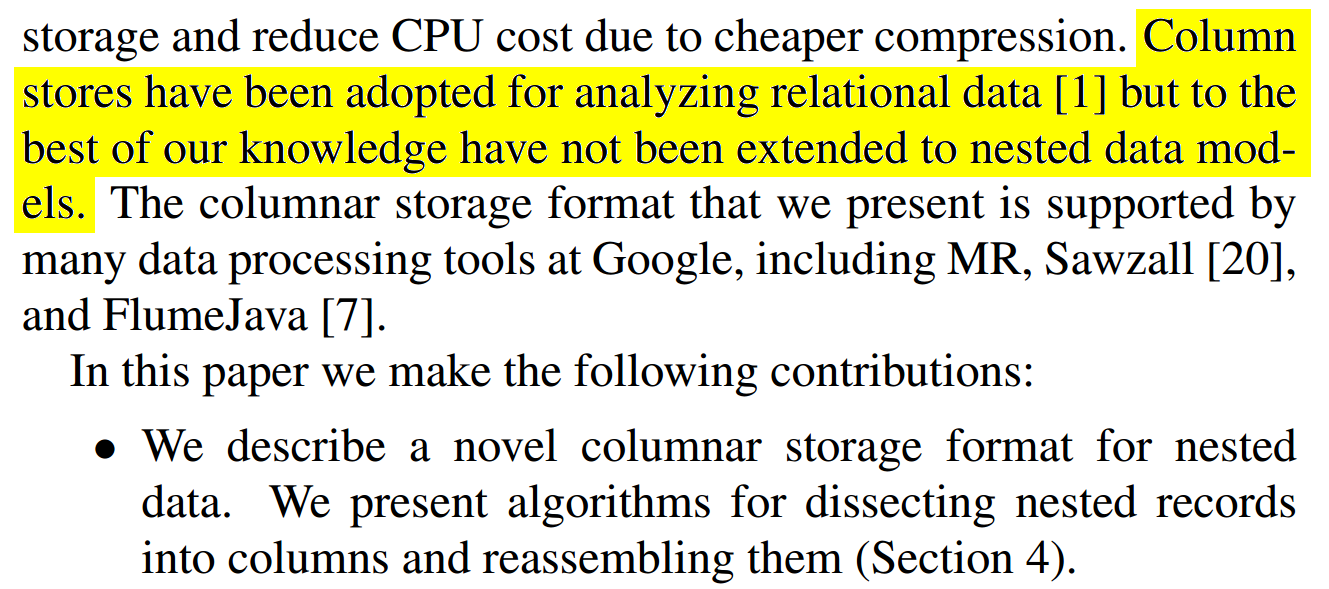
\includegraphics[width=\linewidth]{dremel.png}

\vspace{0.5 cm}
\mbox{ } \hfill \textcolor{darkblue}{\Large Independently developed: this is xenobiology!} \hfill \mbox{ }
\end{frame}

\begin{frame}{Translation dictionary}
\vspace{0.5 cm}
\begin{columns}[t]
\column{0.3\linewidth}
\textcolor{darkblue}{\underline{\large ROOT}}

\vspace{0.2 cm}
\begin{itemize}\setlength{\itemsep}{0.2 cm}
\item Streamer info
\item Splitting
\item Event cluster

\vspace{2\baselineskip}

\item TBuffer

\vspace{\baselineskip}

\item TBasket
\end{itemize}

\column{0.7\linewidth}
\textcolor{darkblue}{\underline{\large Dremel/Parquet}}

\vspace{0.2 cm}
\begin{itemize}\setlength{\itemsep}{0.2 cm}
\item Schema: description of all data types
\item Shredding: breaking objects into columns
\item Row group: group of columns (which may have different lengths) corresponding to a fixed number of rows
\item Column: contiguous data for one scalar leaf of the schema
\item Page: fixed-size chunk of data for one compression pass
\end{itemize}
\end{columns}
\end{frame}

\begin{frame}{Repetition and definition levels}
\vspace{0.5 cm}
\begin{columns}[T]
\column{0.4\linewidth}
\small Schema of primitives that can be scalar or repeated, required or optional.

\vspace{0.2 cm}
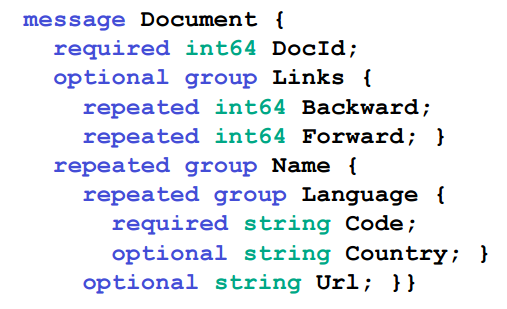
\includegraphics[width=\linewidth]{repetition_and_definition_schema.png}

\vspace{0.1 cm}
All data can be flattened with two extra fields: \mbox{$r$ and $d$.\hspace{-1 cm}}

\vspace{-0.2 cm}

\column{0.5\linewidth}
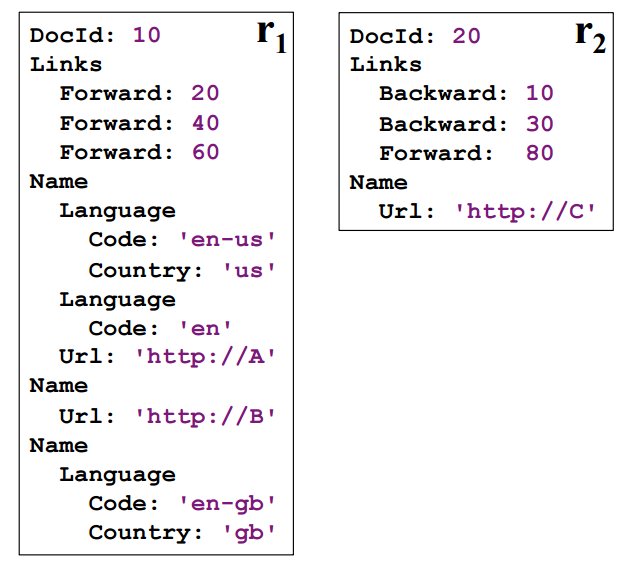
\includegraphics[width=\linewidth]{repetition_and_definition_data.png}
\end{columns}

\vspace{0.5 cm}
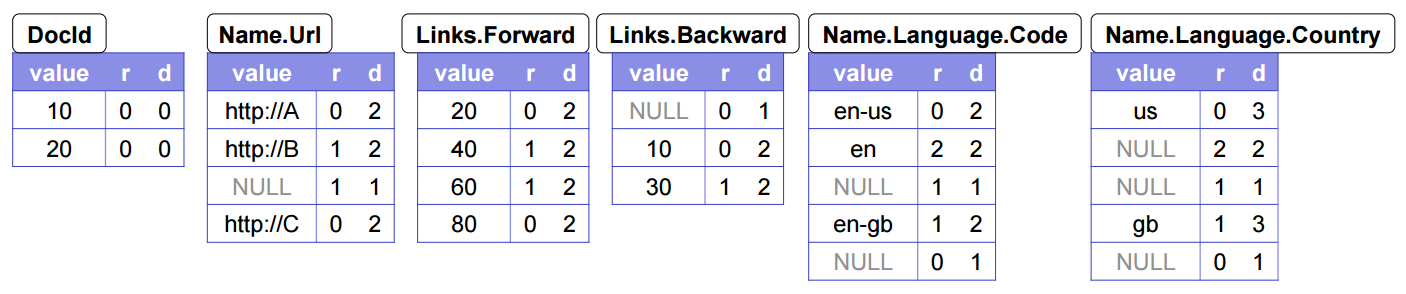
\includegraphics[width=\linewidth]{repetition_and_definition_arrays.png}
\end{frame}

\begin{frame}{Detail on repetition level}
\vspace{0.3 cm}
\textcolor{darkblue}{Given:} \hfill {\tt [} {\tt [} {\tt a} {\tt b} {\tt c} {\tt ]} {\tt [} {\tt d} {\tt e} {\tt f} {\tt g} {\tt ]} {\tt ]} {\tt [} {\tt [} {\tt h} {\tt ]} {\tt [} {\tt i} {\tt j} {\tt ]} {\tt ]}

\textcolor{darkblue}{Data array:} \hfill {\tt \ } {\tt \ } {\tt a} {\tt b} {\tt c} {\tt \ } {\tt \ } {\tt d} {\tt e} {\tt f} {\tt g} {\tt \ } {\tt \ } {\tt \ } {\tt \ } {\tt h} {\tt \ } {\tt \ } {\tt i} {\tt j} {\tt \ } {\tt \ }

\textcolor{darkblue}{Repetition level:} \hfill {\tt \ } {\tt \ } \textcolor{darkorange}{\tt 0} \textcolor{darkgreen}{\tt 2} \textcolor{darkgreen}{\tt 2} {\tt \ } {\tt \ } \textcolor{blue}{\tt 1} \textcolor{darkgreen}{\tt 2} \textcolor{darkgreen}{\tt 2} \textcolor{darkgreen}{\tt 2} {\tt \ } {\tt \ } {\tt \ } {\tt \ } \textcolor{darkorange}{\tt 0} {\tt \ } {\tt \ } \textcolor{blue}{\tt 1} \textcolor{darkgreen}{\tt 2} {\tt \ } {\tt \ }

\begin{center}
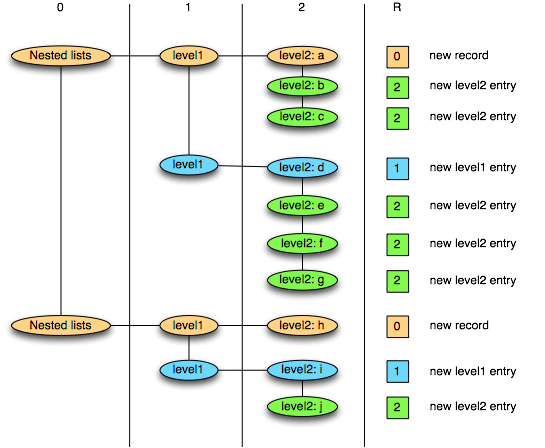
\includegraphics[width=0.73\linewidth]{repetition_and_definition_3.png}
\end{center}
\end{frame}

\begin{frame}{Detail on definition level}
\vspace{0.2 cm}
\begin{center}
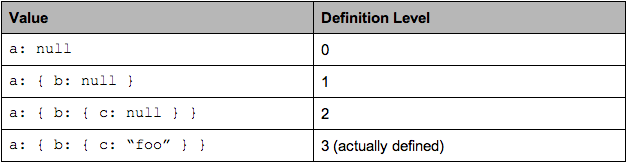
\includegraphics[width=0.85\linewidth]{repetition_and_definition_4.png}

\vspace{0.3 cm}
\mbox{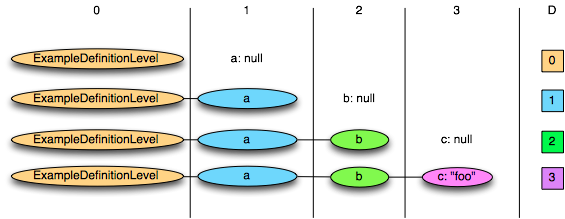
\includegraphics[width=0.8\linewidth]{repetition_and_definition_5.png}\hspace{0.5 cm}}
\end{center}

\vspace{-0.2 cm}
Intended for nullable data (e.g.\ missing values), but also {\it required} to describe empty lists. Can't adopt repetition levels without definition levels.
\end{frame}

\begin{frame}{Comparison to ROOT's counters}
\vspace{0.5 cm}
\begin{columns}[t]
\column{0.5\linewidth}
\textcolor{darkblue}{\underline{\large Dremel/Parquet}}

\begin{itemize}
\item Repetition/definition levels describe arbitrarily deep nesting in one pair of arrays.

\item Maximum possible $r$, $d$ values determined by depth of nesting; can be packed.

\textcolor{darkgrey}{(A depth-1 list of any length can be described by two bits {\it per element.})}

\item Determining list size is a history-dependent calculation.

\end{itemize}

\column{0.5\linewidth}
\textcolor{darkblue}{\underline{\large ROOT}}

\begin{itemize}
\item A separate counter branch would be needed for every level of depth.

\item List length is bounded by the number of bits in the counter.

\textcolor{darkgrey}{(An 8-bit counter is more tightly packed for lists of length 4 through 255.)}

\item List size is readily available.
\end{itemize}
\end{columns}
\end{frame}

\begin{frame}{Best of both for nested lists}
\vspace{0.5 cm}
Can we keep counters but gain the ability to describe arbitrarily deep nesting in one array? Yes!

\vspace{0.2 cm}
\textcolor{red}{\mbox{\hspace{1 cm} $\rightarrow$} Fill the counter recursively.}

\vspace{0.3 cm}
\textcolor{darkblue}{Given:} \hfill {\tt [} {\tt [} {\tt a} {\tt b} {\tt c} {\tt ]} {\tt [} {\tt d} {\tt e} {\tt f} {\tt g} {\tt ]} {\tt ]} {\tt [} {\tt [} {\tt h} {\tt ]} {\tt [} {\tt i} {\tt j} {\tt ]} {\tt ]}

\textcolor{darkblue}{Data array:} \hfill {\tt \ } {\tt \ } {\tt a} {\tt b} {\tt c} {\tt \ } {\tt \ } {\tt d} {\tt e} {\tt f} {\tt g} {\tt \ } {\tt \ } {\tt \ } {\tt \ } {\tt h} {\tt \ } {\tt \ } {\tt i} {\tt j} {\tt \ } {\tt \ }

\textcolor{darkblue}{Recursive counter:} \hfill \textcolor{darkorange}{\tt 2} \textcolor{blue}{\tt 3} {\tt \ } {\tt \ } {\tt \ } {\tt \ } \textcolor{blue}{\tt 4} {\tt \ } {\tt \ } {\tt \ } {\tt \ } {\tt \ } {\tt \ } \textcolor{darkorange}{\tt 2} \textcolor{blue}{\tt 1} {\tt \ } {\tt \ } \textcolor{blue}{\tt 2} {\tt \ } {\tt \ } {\tt \ } {\tt \ }

\vspace{0.3 cm}
\begin{itemize}
\item Lossless: we know to interpret the \textcolor{darkorange}{orange} numbers as first-level and the \textcolor{blue}{blue} numbers as second-level by reading it left to right (history dependent calculation).

\item Backward compatible with ROOT's counters.

\item Data array is now completely split; we can apply vectorized functions to it (e.g.\ GPU).
\end{itemize}
\end{frame}

\begin{frame}[fragile]{A more complex example}
\vspace{0.5 cm}
\mbox{\hspace{-0.5 cm}Consider a schema that mixes arrays and structs:}
\begin{columns}
\column{0.3\linewidth}
\scriptsize
\begin{minted}{scala}
class Inner(
  a: Double,
  b: List[Double]
)
class Outer(
  x: Double,
  y: List[Inner]
)
\end{minted}

\column{0.5\linewidth}
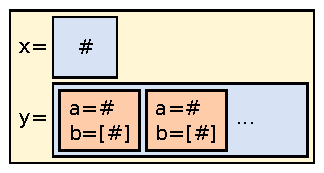
\includegraphics[width=\linewidth]{record.pdf}
\end{columns}

\vspace{0.3 cm}
{\hspace{-0.5 cm}\begin{minipage}{\linewidth}
{\normalsize Data like this:}

\small
\begin{minted}{python}
Outer(x=1, y=[Inner(a=2, b=[ 3,  4]), Inner(a=5, b=[])])
Outer(x=6, y=[Inner(a=9, b=[10, 11])                  ])
\end{minted}

\vspace{0.2 cm}
{\normalsize Only needs a counter for each leaf with different structure:}

\vspace{-0.2 cm}
\begin{columns}[b]
\column{0.3\linewidth}
\small
\begin{verbatim}
x:   [1, 6]
y.a: [2, 5, 9]
y.b: [3, 4, 10, 11]
\end{verbatim}

\column{0.4\linewidth}
\small
\begin{verbatim}
y.a@size: [2, 1]
y.b@size: [2, 2, 0, 1, 2]
\end{verbatim}
\end{columns}
\end{minipage}}
\end{frame}

% the zig-zag integer trick

% abstract types
% Datashape

\end{document}
